\chapter{Results}
This chapter shows the results for the following experiments.
% Reconstruction quality is mean of PSNR of images inside and outside of
% the training sets.
\begin{enumerate}
 \item Convergence of reconstruction quality for different training parameters
(block size, learning coefficients).
 \item Comparison of reconstruction quality of dictionaries
in single and in cluster runs. 
 \item Comparison of compression quality between learned dictionaries, JPEG and
JPEG2000  on natural images and sketches.
 \item Observations of structures of dictionary atoms from different
groups of images and block sizes.
\end{enumerate}

We discuss the results in the next chapter.

\newpage
%\section{Quality}
%\subsection*{trained vs. analytical base}
%\subsection*{Compression ratio}
%\subsection*{Dictionary size}
%Setup:
%  initialize: random pixels, radom samples 
%  dict size: 256, 1000, 4000, 8000
%  coeffs: 5, 10, 20

\section{Training parameters}
\begin{figure}[h]
\centering
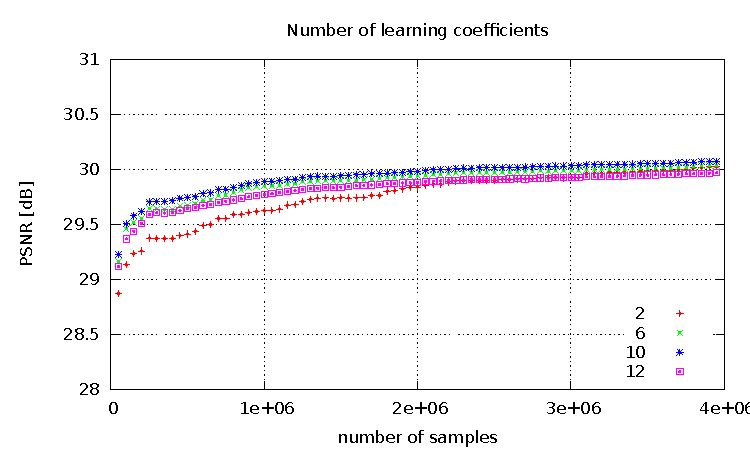
\includegraphics[width = 0.8\textwidth]{../tests/results/coeffsConverg.pdf}
\caption{reconstruction quality for different training coefficients}
\label{fig:dict size}
\end{figure}

\begin{figure}[h]
\centering
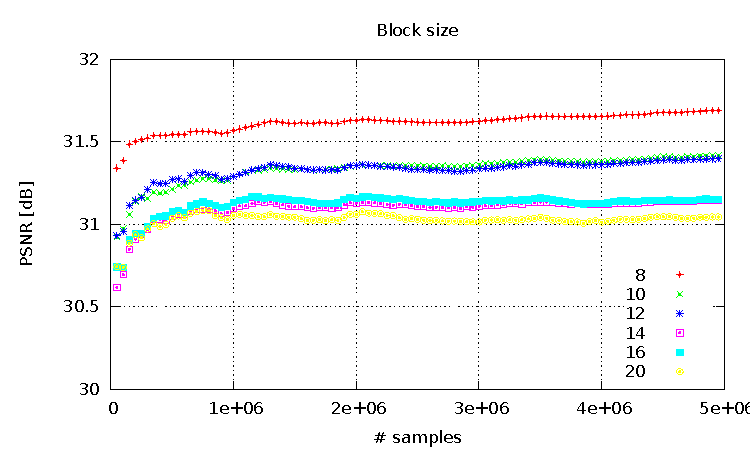
\includegraphics[width = 0.8\textwidth]{../tests/results/blockSizeConverg.pdf}
\caption{reconstruction quality for different block sizes}
\label{fig:dict size}
\end{figure}

% \begin{table}[h]
% \caption{dictionary size}
% \centering
% \begin{tabular}{l  c  c  c  c  c}
% \toprule
% Image & 1 & 2 & 3 & 4 & 5 \\
% \hline
% 300 & 30 & 30 & 30 & 30 & 30 \\
% 600 & 30 & 30 & 30 & 30 & 30 \\
% 900 & 30 & 30 & 30 & 30 & 30 \\
% 1800 & 30 & 30 & 30 & 30 & 30 \\
% 3000 & 30 & 30 & 30 & 30 & 30 \\
% \bottomrule
% \end{tabular}
% \end{table}

\newpage
\section{Dictionary size}

\begin{figure}[h]
\centering
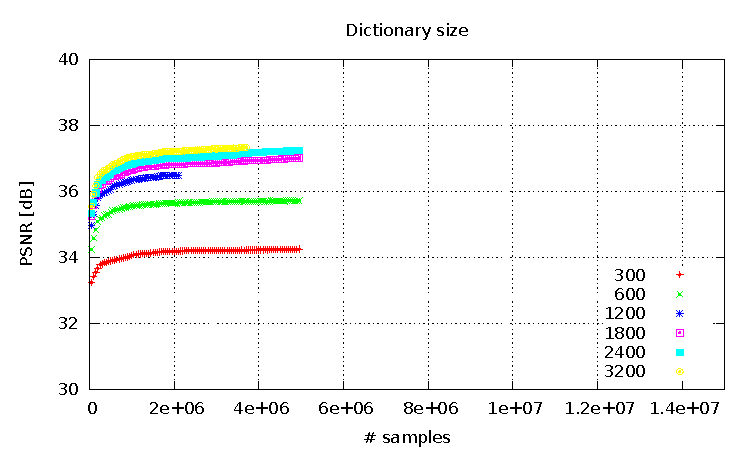
\includegraphics[width = 0.8\textwidth]{../tests/results/dictSizeOMP.pdf}
\caption{reconstruction quality for different dictionary sizes (OMP)}
\label{fig:dict size}
\end{figure}

\begin{figure}[h]
\centering
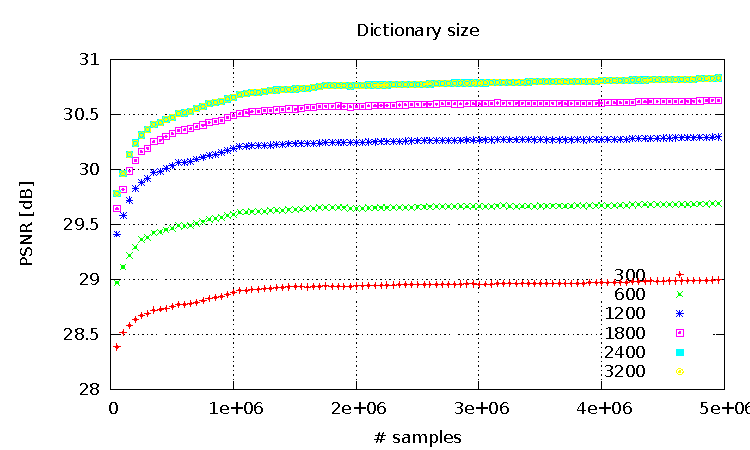
\includegraphics[width = 0.8\textwidth]{../tests/results/dictSizeLasso.pdf}
\caption{reconstruction quality for different dictionary sizes (Lasso)}
\label{fig:dict size}
\end{figure}

% \begin{table}[H]
% \caption{single vs. cluster}
% \centering
% \begin{tabular}{l c c c c c}
% \hline\hline
% Image & 300 & 600 & 900 & 1800 & 3000 \\
% \hline
% image 1 & 30 & 30 & 30 & 30 & 30 \\
% image 2 & 30 & 30 & 30 & 30 & 30 \\
% image 3 & 30 & 30 & 30 & 30 & 30 \\
% \hline
% \end{tabular}
% \end{table}

\newpage
\section{Compression}
\subsection{Natural images}


32.3438

\begin{table}[H]
%\caption{single vs. cluster}
\centering
\begin{tabular}{| l c | c | c | c|}
\hline\hline
Image & bpp & SPRS & JPEG & JPEG2000 \\
\hline
image 1 & 1.12 & 31.2205 & 32.3289 & 36.613 \\
image 2 & 1.01 & 34.7735 & 35.0671 & 40.3299 \\
image 3 & 1.8  & 29.0597 & 27.2556 & 31.7412 \\
image 4 & 0.74  & 35.9499 & 35.5104 & 39.4195 \\

\hline
\end{tabular}
\end{table}

\begin{figure}[H]
\centering
\subfloat[sprs ]{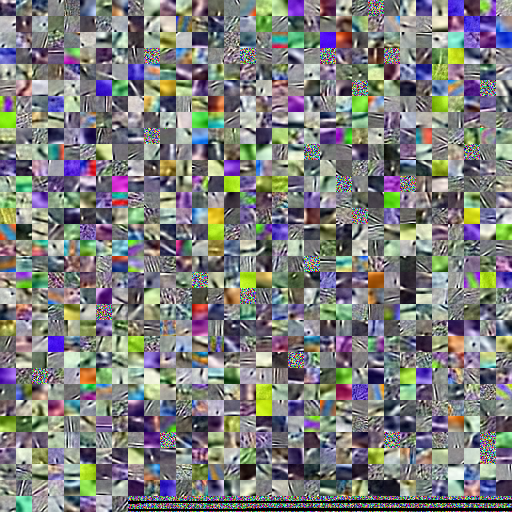
\includegraphics[width =
0.3\textwidth]{images/16_1000_1000_10_lasso.png}}
\hspace{5mm}
\subfloat[JPEG]{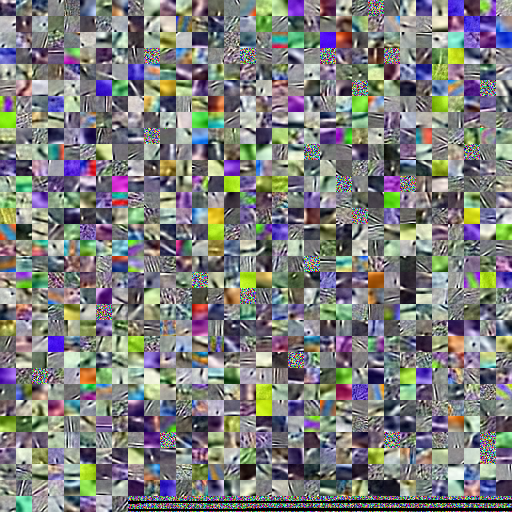
\includegraphics[width =
0.3\textwidth]{images/16_1000_1000_10_lasso.png}}
\hspace{5mm}
\subfloat[JPEG2000]{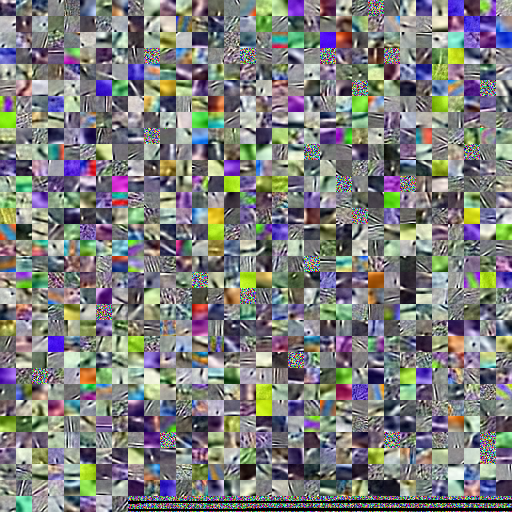
\includegraphics[width =
0.3\textwidth]{images/16_1000_1000_10_lasso.png}}
%\caption{}
%\label{fig:16_1000_lasso}
\end{figure}

\begin{figure}[H]
\centering
\subfloat[sprs]{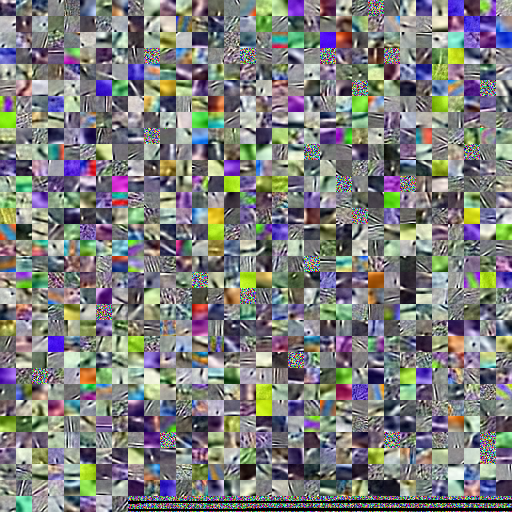
\includegraphics[width =
0.3\textwidth]{images/16_1000_1000_10_lasso.png}}
\hspace{5mm}
\subfloat[JPEG]{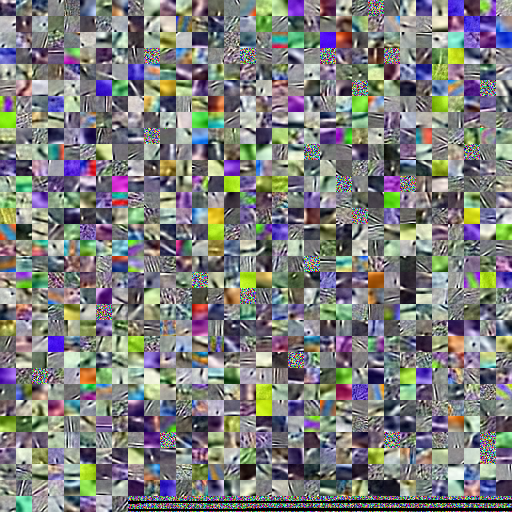
\includegraphics[width =
0.3\textwidth]{images/16_1000_1000_10_lasso.png}}
\hspace{5mm}
\subfloat[JPEG2000]{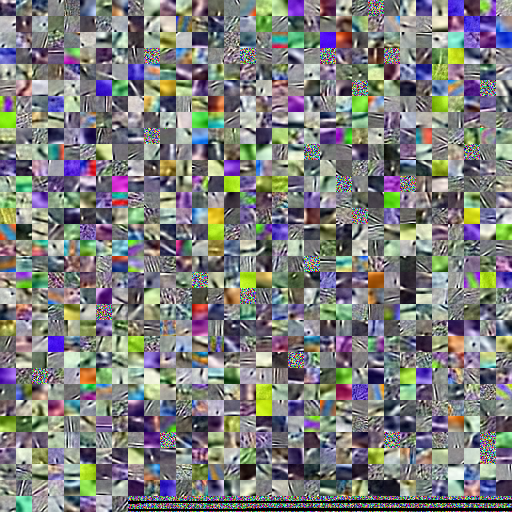
\includegraphics[width =
0.3\textwidth]{images/16_1000_1000_10_lasso.png}}
%\caption{}
%\label{fig:16_1000_lasso}
\end{figure}



\newpage
\subsection{Sketches}

\begin{table}[H]
%\caption{single vs. cluster}
\centering
\begin{tabular}{| l c | c | c | c|}
\hline\hline
Image & bpp & SPRS & JPEG & JPEG2000 \\
\hline
sketch 1 & 0.084 & 33.9594 & 28.9578 & 38.3258  \\
sketch 2 & 0.13 & 32.9 & 34.5546 &  40.0159 \\
sketch 3 & 0.08 & 32.5131 & 28.6558 & 36.3093  \\
\hline
\end{tabular}
\end{table}

\begin{figure}[H]
\centering
\subfloat[sprs]{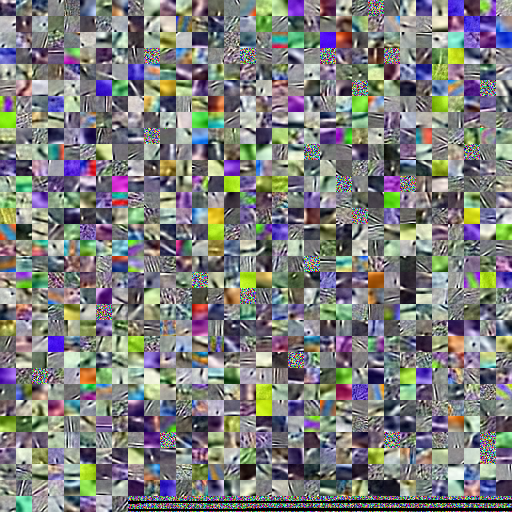
\includegraphics[width =
0.3\textwidth]{images/16_1000_1000_10_lasso.png}}
\hspace{5mm}
\subfloat[JPEG]{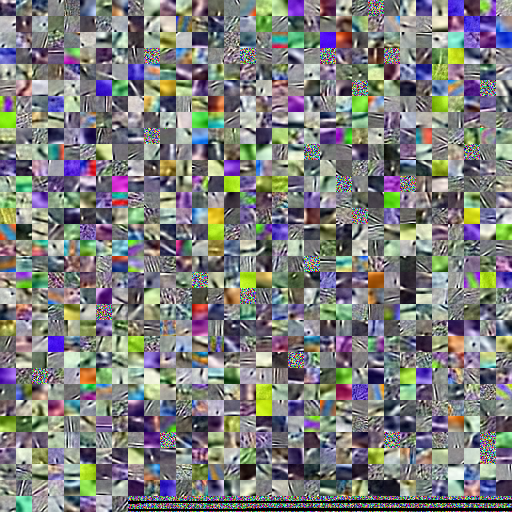
\includegraphics[width =
0.3\textwidth]{images/16_1000_1000_10_lasso.png}}
\hspace{5mm}
\subfloat[JPEG2000]{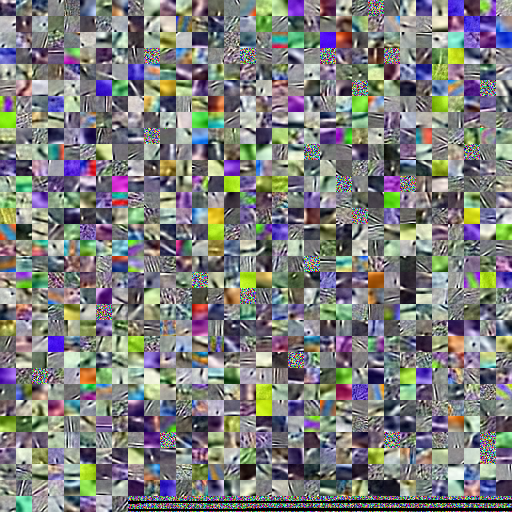
\includegraphics[width =
0.3\textwidth]{images/16_1000_1000_10_lasso.png}}
%\caption{}
%\label{fig:16_1000_lasso}
\end{figure}

\begin{figure}[H]
\centering
\subfloat[sprs]{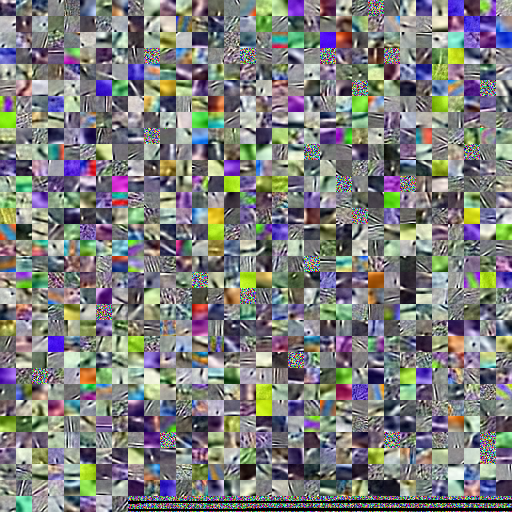
\includegraphics[width =
0.3\textwidth]{images/16_1000_1000_10_lasso.png}}
\hspace{5mm}
\subfloat[JPEG]{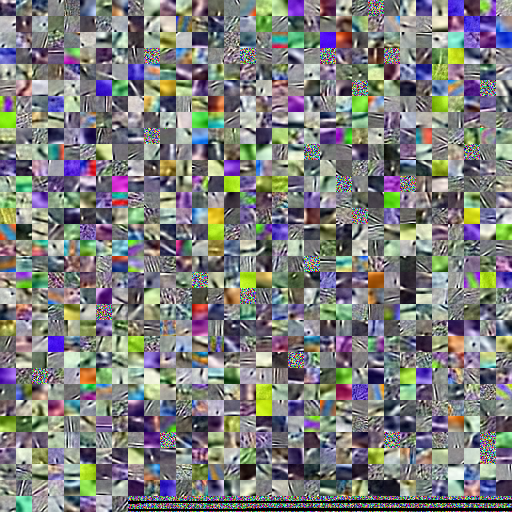
\includegraphics[width =
0.3\textwidth]{images/16_1000_1000_10_lasso.png}}
\hspace{5mm}
\subfloat[JPEG2000]{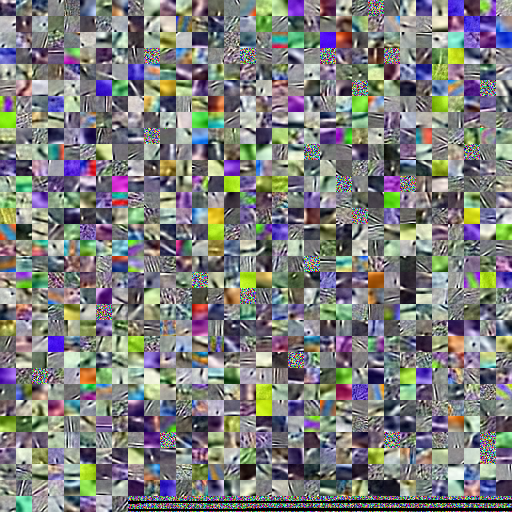
\includegraphics[width =
0.3\textwidth]{images/16_1000_1000_10_lasso.png}}
%\caption{}
%\label{fig:16_1000_lasso}
\end{figure}



\newpage
\section{Dictionary elements}
\begin{figure}[H]
\centering
\subfloat{
\includegraphics[width = 0.3\textwidth]{images/gradient.png}}
\hspace{5mm}
\subfloat{
\includegraphics[width = 0.3\textwidth]{images/checkerboard.png}}
\hspace{5mm}
\subfloat{
\includegraphics[width = 0.3\textwidth]{images/spot.png}}
\hspace{5mm}
\subfloat{
\includegraphics[width = 0.3\textwidth]{images/edges.png}}
\hspace{5mm}
\subfloat{
\includegraphics[width = 0.3\textwidth]{images/wavelet.png}}
\caption{image from database}
\label{fig:USC-SIPI}
\end{figure}





